\section{W : Algorithms III - Huffman/Strings}
\label{chap:algos3}

%%%%%%%%%%%%%%%%%%%%%%%%%%%%%%%%%%%%%%%%%%%%%%%%%%%%%%%%%%%%%

\begin{frame}[fragile]
\frametitle{Algorithm : Huffman Compression}
\begin{columns}[T]

\begin{column}{0.45\textwidth}
\begin{itemize}[<+->]
\item Often we wish to compress data, to reduce storage requirements, or to speed transmission.
\item  Text is particularly suited to compression since using one byte per character is wasteful - some letters occur much more frequently.
\item  Need to give frequently occurring letters short codes, typically a few bits. Less common letters can have long bit patterns.
\end{itemize}
\end{column}

\begin{column}{0.45\textwidth}
\begin{itemize}[<+->]
\item To encode the string "BABBAGE":

\vspace*{2ex}
\pause
\begin{center}
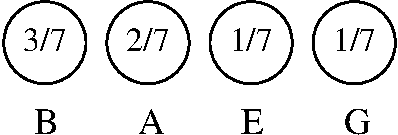
\includegraphics[width=0.6\textwidth]{../Images/huff1.pdf}
\end{center}
\item Keep a list of characters, ordered by their frequency
\end{itemize}
\end{column}

\end{columns}
\end{frame}

%%%%%%%%%%%%%%%%%%%%%%%%%%%%%%%%%%%%%%%%%%%%%%%%%%%%%%%%%%%%%%

\begin{frame}[fragile]
\frametitle{Huffman Compression II}
\begin{columns}[T]

\begin{column}{0.45\textwidth}
\begin{itemize}[<+->]
\item Use the two least frequent to form a sub-tree, and re-order (sort) the nodes~:

\pause
\vspace*{2ex}
\begin{center}
\includegraphics[width=0.6\textwidth]{../Images/huff2.pdf}
\end{center}
\end{itemize}
\end{column}

\pause
\begin{column}{0.45\textwidth}
\begin{center}
\includegraphics[width=0.6\textwidth]{../Images/huff3.pdf}
\end{center}
\pause
\begin{itemize}[<+->]
\item A = 10, B = 0, E = 110, G = 111
\item String stored using 13 bits.
\end{itemize}
\end{column}

\end{columns}
\end{frame}

%%%%%%%%%%%%%%%%%%%%%%%%%%%%%%%%%%%%%%%%%%%%%%%%%%%%%%%%%%%%%%

\begin{frame}[fragile]
\frametitle{Algorithm : Rabin-Karp String Searching}
\begin{columns}[T]

\begin{column}{0.40\textwidth}
\begin{itemize}[<+->]
\item The task of searching for a string amongst a large
amount of text is commonly required in word-processors,
but more interestingly in massive Biological Databases e.g.\ searching for amino acids in protein sequences.
\item How difficult can it be~? Don't you just do a character by
character brute-force search~?
\begin{verbatim}
Master String : AAAAAAAAAAAAH
Substring     : AAAAAAH
Substring     :  AAAAAAH
Substring     :   AAAAAAH
\end{verbatim}
\end{itemize}
\end{column}

\pause
\begin{column}{0.50\textwidth}
\begin{itemize}[<+->]
\item If the master string has $m$ characters, and the search string has $n$ characters then this search has complexity: $O(mn)$
\item Recall that to compute a hash function on a word we did something like:
\[
h("NEILL") =
\]
{\scriptsize
\[
(13\times26^4 + 4\times26^3 + 8\times26^2 + 11\times26 + 11) \% P
\]
}
where $P$ is a big prime number.
\item This can be expanded by Horner's method to:
{\scriptsize
\[
(((((((13\times26)+ 4)\times26) + 8)\times26) + 11)\times26 + 11) \% P
\]
}
\end{itemize}
\end{column}

\end{columns}
\end{frame}

%%%%%%%%%%%%%%%%%%%%%%%%%%%%%%%%%%%%%%%%%%%%%%%%%%%%%%%%%%%%%%

\begin{frame}[fragile]
\frametitle{Rabin-Karp II}
\begin{columns}[T]

\begin{column}{0.530\textwidth}
\begin{itemize}[<+->]
\item For a large search string, overflow can occur. We therefore move the {\it mod} operation inside the brackets:
{\scriptsize
\[
((((((13\times26)+ 4)\%P \times26) + 8)\%P \times26) + 11)\%P \times26 + 11) \% P
\]
}
\item We can compute a hash number for the search string, and for the initial part of the master string.
\item When we compute the hash number for the next part of the master, most of the computation is common, we just need to take out the effect of the first letter and add in the effect of the new one.
\item One small calculation each time we move one place right in the master.
\item Complexity $O(m+n)$ roughly, but need to check that two identical hash numbers really has identified two identical strings.
\end{itemize}
\end{column}

\pause
\begin{column}{0.420\textwidth}
\lstinputlisting[style=basicc]{../Code/ChapW/rabinkarp.c}
\end{column}

\end{columns}
\end{frame}

%%%%%%%%%%%%%%%%%%%%%%%%%%%%%%%%%%%%%%%%%%%%%%%%%%%%%%%%%%%%%%

\begin{frame}[fragile]
\frametitle{Algorithm : Boyer-Moore String Searching}
\begin{columns}[T]

\begin{column}{0.45\textwidth}
The Boyer-Moore algorithm uses (in part) an array flagging
which characters form part of the search string and an array telling
us how far to slide right if that character appears in the master and causes
a mismatch.

\outputlisting{../Code/ChapW/boyermoore_ex1.txt}
\end{column}

\pause
\begin{column}{0.45\textwidth}
\begin{itemize}[<+->]
\item With a right-to-left walk through the search string we see that the G and the R mismatch on the first comparison.
\item Since R doesn't appear in the
search string, we can take $5$ steps to the right.
\item The next comparison is between the G and the S. We can slide the search string right until it matches the S in the master.
\end{itemize}
\end{column}

\end{columns}
\end{frame}

%%%%%%%%%%%%%%%%%%%%%%%%%%%%%%%%%%%%%%%%%%%%%%%%%%%%%%%%%%%%%%

\begin{frame}[fragile]
\frametitle{Boyer-Moore II}
\begin{columns}[T]

\begin{column}{0.45\textwidth}
\outputlisting{../Code/ChapW/boyermoore_ex2.txt}
\end{column}

\begin{column}{0.45\textwidth}
\begin{itemize}[<+->]
\item Now the C doesn't appear in the master and once again we can slide a full $5$ places to the right.
\item After $3$ more full slides right we arrive at the T in CONSISTING.
\item We align the T's, and have found our match using $7$ compares (plus $5$ to verify the match).
\end{itemize}
\end{column}

\end{columns}
\end{frame}















